\begin{figure}[H]
\begin{center}
    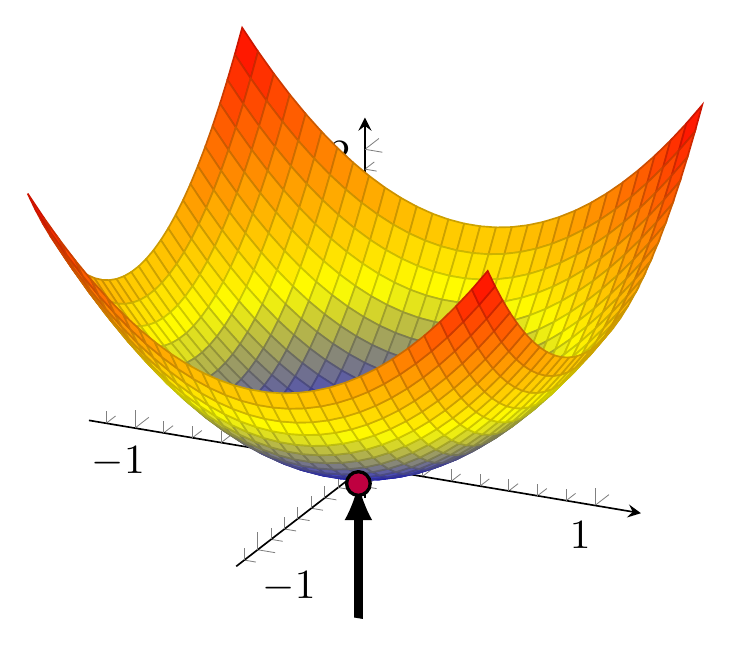
\begin{tikzpicture}[scale=1.5]
    %\draw[step=.5, gray!40, very thin] (0,0) grid (8,4);
\begin{axis}[axis lines=center,
       enlargelimits,
       tick align=inside,
       domain=-1:1,
       samples=30,
       minor tick num=7,]		
       \addplot3 [surf]{x^2+y^2};
       \draw[arrows=-latex,line width=2pt] (2.8cm,-5.2cm) -- (2.8cm,.23cm);
       \draw[thick,fill=purple] (2.8cm,.23cm) circle (0.1cm);
\end{axis}
\end{tikzpicture}
\caption{Gradient Decent }\label{fig:gradient_decent_surf}
\end{center}
\end{figure} 